% OWD 2024: IMLO assignment report
%
\documentclass[journal]{IEEEtran}
\usepackage[en-GB]{datetime2}
\usepackage{xcolor, amsmath, amssymb, tikz, nidanfloat}
\usepackage[
    colorlinks,
    linkcolor={red!50!black},
    citecolor={blue!50!black},
    urlcolor={blue!80!black}
]{hyperref}

\usetikzlibrary{positioning, fit}

\newcommand\dotsep{\enspace\textperiodcentered\enspace}
\newcommand\networkperformance{43}
\DeclareMathOperator\relu{\mathsf{ReLU}}
\DeclareMathOperator\batchnorm{\mathsf{BNorm}}
\DeclareMathOperator\linear{\mathsf{Lin}}
\DeclareMathOperator\celoss{\mathsf{CELoss}}
\DeclareMathOperator\convol{\mathsf{Conv2d}}
\DeclareMathOperator\weight{\mathsf{Weight}}
\DeclareMathOperator\maxpool{\mathsf{MaxPool2d}}
\DeclareMathOperator\bias{\mathsf{Bias}}

\title{Classification of the 102-Category \emph{Flowers} Dataset with
    Convolutional Deep Neural Networks}
\author{Examination Candidate \#Y3898772%
    \thanks{Manuscript prepared with \LaTeX\ and \texttt{IEEEtran} on \today.}}

\IEEEspecialpapernotice{Submitted in partial fulfilment of the requirements of
    the \href{https://www.york.ac.uk/students/studying/manage/programmes/%
    module-catalogue/module/COM00026I/2023-24}{\emph{Intelligent Systems:
    Machine Learning and Optimisation}} module assignment at the University of
    York in the 2023/24 academic year.\vspace{-2ex}}

\begin{document}
\maketitle
\begin{abstract}
    The classification of data into discrete categories is an ancient problem,
    recently made accessible on extremely large datasets due to substantial
    advances in hardware capability; one such advancement is the introduction of
    graphics processing units (GPUs) in machine learning applications,
    particularly for the training and evaluation of deep neural networks (DNNs).
    This report defines and evaluates such a DNN for the classification of the
    102-category \emph{Flowers} dataset%
    \footnote{\url{https://www.robots.ox.ac.uk/~vgg/data/flowers/102/}} from the
    Visual Geometry Group at the University of Oxford.

    For this purpose, a convolutional deep neural network (CDNN) was
    constructed, using topical understandings of batch normalisation (BN)
    techniques for regularisation. A fair 102-sided die would classify an
    arbitrarily chosen \emph{Flowers} image in $\mathbf{0.98}$\% of instances,
    whereas the constructed CDNN achieves $\mathbf{\networkperformance}$\%
    accuracy on the test data split.
\end{abstract}
\section{Introduction}
\IEEEPARstart{C}{lassical} classification-based computer vision problems are
concerned with the training of DNNs to categorise images by a fixed set of
`labels'. Often, this involves recognising images from a wide range of highly
disjointed categories, and significant work and experimentation has been
conducted in this area \cite{Chen:2021}. In contrast to many existing datasets,
the 102-category \emph{Flowers} set consists of a large number of relatively
similar categories, each representing a genus of flower that is commonly found
on the British Isles \cite{Nilsback:2008}. Given the similarity between the
categories, coupled with the relatively small volume of training
data\footnote{Training: 1020 images; Validation: 1020 images; Testing: 6149
images.}, the \emph{Flowers} dataset presents a notably difficult problem.

Previous experiments utilising support vector machines (SVMs) equipped with
weighted linear combinations of numerous kernels can attain impressive
test-accuracies of up to $72.8$\% \cite{Nilsback:2008}, where the optimum
weights can be systematically learned \cite{Varma:2007}. Subsequently developed
models based on \emph{Inception-v3}, trained with the 14-million-sample
\emph{ImageNet} dataset, have achieved an impressive $94$\% test-accuracy on
\emph{Flowers} \cite{Xia:2017}.

As the capabilities of machine learning advance, and demand increases, the
complexity of the datasets on which neural networks are expected to work will
invariably rise, thus giving justification to the importance of research into
the systematic learning of large-category datasets, often with restricted
volumes of training samples.  The DNN presented henceforth uses a combination of
convolutions, batch normalisation, the rectified linear activation function,
cross-entropy-softmax loss, and learning-rate scheduling to attain a
test-accuracy of $\networkperformance$\% with no pre-trained information.

\section{Method}
The designed CDNN follows a typical convolutional process: given a batch of
three-channel (RGB) images each representable as tensors over $\mathbb{Q}_+$,
the CDNN passes the batch through a sequence of hidden layers:
\begin{enumerate}
    \item Using a $3 \times 3$ kernel, perform two-dimensional convolution over
        the three-channel input to produce a 32-channel output. Iterate
        over all batch images; \label{item:method-first-stage}
    \item Execute batch-normalisation on the 32-channel tensor;
    \item Activate the batch-normalised tensor with the rectified linear unit
        activation function; and
    \item Perform two-dimensional max-pooling on the output with a $2$-stride $2
        \times 2$ kernel. \label{item:method-last-stage}
    \item Repeat stages \ref{item:method-first-stage} to
        \ref{item:method-last-stage} with increasing numbers of input-output
        convolution channels: $32 \to 64$ and $64 \to 128$, to yield a
        128-channel convolved tensor, which has been normalised, activated, and
        pooled;
    \item Linearise the feature map using a four-stage process to create a
        102-component probability tensor for each image in the batch.
\end{enumerate}
Each aspect of these hidden layers, and the cross-entropy-softmax loss function,
is now explored in detail.

\subsection{Two-Dimensional Convolution}
On a single $C_\text{in}$-channel image of dimensions
$W_\text{in}$-by-$H_\text{in}$, the two-dimensional convolution operator
$\convol$ is such that
\begin{equation}
    \convol \colon
        \mathbb{Q}^{\left( C_\text{in}, H_\text{in}, W_\text{in} \right)}_+ \to
        \mathbb{Q}^{\left( C_\text{out}, H_\text{out}, W_\text{out} \right)}_+,
\end{equation}
where, for all tensors $\mathcal{A} \in \mathbb{Q}^{\left( C_\text{in},
H_\text{in}, W_\text{in} \right)}_+$ containing channels $\mathcal{A}_1, \ldots,
\mathcal{A}_{C_\text{in}}$,
\begin{equation}
    \mathcal{A} \mapsto \sum_{i=1}^{C_\text{in}} \left[
            \weight\left(C_\text{out}, i\right) \star \mathcal{A}_i
        \right] + \bias(C_\text{out}).
    \label{eqn:convolution}
\end{equation}
(The convolutional cross-correlation operator is denoted by $\star$, and
$\weight$ and $\bias$ select the suitable channel-wise weight and global bias
respectively.) All $C_\text{out}$ two-dimensional components of the codomain
of $\convol$, $\mathbb{Q}^{\left( C_\text{out}, H_\text{out}, W_\text{out}
\right)}_+$, are a \emph{feature maps} of the convolution.
Convolution is an important stage of the feature-extraction process, whereby
unimportant features are abstracted away from the attention of the learnable
parameters of the CDNN. Kernel sizes of $3 \times 3$ were selected empirically,
and based on the relevant literature \cite{Wang:2016}.

\subsection{Batch Normalisation (BN)}
BN, typically performed on the convolved tensor, causes faster convergence of
the CDNN\footnotemark. Normalisation as a pre-processing technique is known to
substantially improve the performance of a DNN, and BN extends the processing to
each hidden layer of the network. Equation \eqref{eqn:batch-norm} represents the
transformation of the convoluted batch-tensor $\mathcal{B}$, where
$\mu_\mathcal{B}$ and $\sigma_\mathcal{B}$ denote the mean and standard
deviation of $\mathbb{Q}$-components of $\mathcal{B}$ respectively; $\gamma$ and
$\beta$ represent shift parameters of the standard deviation and mean
respectively \cite{Laarhoven:2017}.
\begin{equation}
    \batchnorm(\mathcal{B}) = \frac{%
        \gamma\left(\mathcal{B}-\mu_\mathcal{B}\right)}
    {\sigma_\mathcal{B}} + \beta \label{eqn:batch-norm}
\end{equation}
Given the known regularising properties of BN \cite{Luo:2019}, no further
techniques were employed to discourage over-fitting.
\footnotetext{The usefulness of BN was originally thought to be explained by its
supposed tenancy to reduce the DNN's \emph{internal covariate shift} (ICS)
\cite{Ioffe:2015}. In a groundbreaking 2019 study, it was shown that BN improves
the \emph{$\beta$-Lipschitzness} of the derivative of the cost function, hence
smoothening the cost function, enabling larger learning rates during gradient
descent \cite{Santurkar:2019}.}

\subsection{Activation with the Rectified Linear Unit}
\subsection{Max-Pooling}
\subsection{Linearisation}
\subsection{Cross-Entropy Loss with Softmax}

\section{Network Architecture}
Figure \ref{fig:network-architecture} is a diagrammatic representation of the
CDNN architecture.
\begin{figure*}[t]
    \centering%
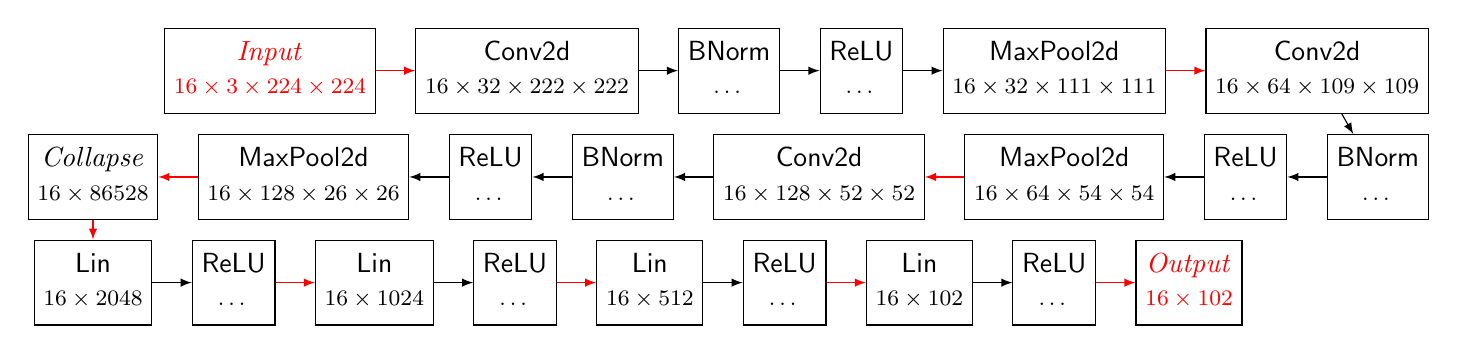
\begin{tikzpicture}
    \newlength\hpad
    \newlength\vpad
    \newlength\hvpad
    \setlength\hpad{.5cm}
    \setlength\vpad{.25cm}
    \setlength\hvpad{1.35cm}
    \colorlet{emphasis-red}{red} % Might need dulling, e.g. 'red!70!black'
    \newcommand*\nodetable[2]{%
        \begin{tabular}{@{}c@{}}%
            #1 \\
            \footnotesize #2%
        \end{tabular}%
    }

    \begin{scope}[every node/.append style={draw, minimum height=2em}]
        % INPUT LAYER
        \node (in) {\color{emphasis-red}%
            \nodetable{\emph{Input}}{$16 \times 3 \times 224 \times 224$}};

        % LAYER #1
        \node [right = \hpad of in] (conv1) {
            \nodetable{$\convol$}{$16 \times 32 \times 222 \times 222$}};
        \node [right = \hpad of conv1] (bn1) {
            \nodetable{$\batchnorm$}{\ldots}};
        \node [right = \hpad of bn1] (relu1) {
            \nodetable{$\relu$}{\ldots}};
        \node [right = \hpad of relu1] (pool1) {
            \nodetable{$\maxpool$}{$16 \times 32 \times 111 \times 111$}};

        % LAYER #2
        \node [right = \hpad of pool1] (conv2) {
            \nodetable{$\convol$}{$16 \times 64 \times 109 \times 109$}};
        \node [below = \hvpad of conv2.east, anchor=east] (bn2) {
            \nodetable{$\batchnorm$}{\ldots}};
        \node [left = \hpad of bn2] (relu2) {
            \nodetable{$\relu$}{\ldots}};
        \node [left  = \hpad of relu2] (pool2) {
            \nodetable{$\maxpool$}{$16 \times 64 \times 54 \times 54$}};

        % LAYER #3
        \node [left =  \hpad of pool2] (conv3) {
            \nodetable{$\convol$}{$16 \times 128 \times 52 \times 52 $}};
        \node [left = \hpad of conv3] (bn3) {
            \nodetable{$\batchnorm$}{\ldots}};
        \node [left = \hpad of bn3] (relu3) {
            \nodetable{$\relu$}{\ldots}};
        \node [left = \hpad of relu3]  (pool3) {
            \nodetable{$\maxpool$}{$16 \times 128 \times 26 \times 26$}};

        % COLLAPSE LAYER
        \node [left = \hpad of pool3] (collapse) {
            \nodetable{\emph{Collapse}}{$16 \times 86528$}};

        % LAYER #4
        \node [below = \vpad of collapse] (lin1) {
            \nodetable{$\linear$}{$16 \times 2048$}};
        \node [right = \hpad of lin1] (relu4) {
            \nodetable{$\relu$}{\ldots}};

        % LAYER #5
        \node [right = \hpad of relu4] (lin2) {
            \nodetable{$\linear$}{$16 \times 1024$}};
        \node [right = \hpad of lin2] (relu5) {
            \nodetable{$\relu$}{\ldots}};

        % LAYER #5
        \node [right = \hpad of relu5] (lin3) {
            \nodetable{$\linear$}{$16 \times 512$}};
        \node [right = \hpad of lin3] (relu6) {
            \nodetable{$\relu$}{\ldots}};

        % LAYER #6
        \node [right = \hpad of relu6]  (lin4) {
            \nodetable{$\linear$}{$16 \times 102$}};
        \node [right = \hpad of lin4]  (relu7) {
            \nodetable{$\relu$}{\ldots}};

        % OUTPUT LAYER
        \node [right = \hpad of relu7] (out) {\color{emphasis-red}%
            \nodetable{\emph{Output}}{$16 \times 102$}};
    \end{scope}

    % Draw CONV-BN-RELU-POOL layer intra-layer arrows
    \foreach \layeridx in {1, 2, 3} {
        \draw[-latex] (conv\layeridx) -- (bn\layeridx);
        \draw[-latex] (bn\layeridx)   -- (relu\layeridx);
        \draw[-latex] (relu\layeridx) -- (pool\layeridx);
    }

    % Inter-layer arrows for CONV-BN-RELU-POOL layers
    \draw[-latex, emphasis-red] (pool1) --    (conv2);
    \draw[-latex, emphasis-red] (pool2) --    (conv3);
    \draw[-latex, emphasis-red] (pool3) --    (collapse);
    \draw[-latex, emphasis-red] (collapse) -- (lin1);

    % Draw LIN-RELU layer intra-layer arrows
    \foreach \linidx/\reluidx in {1/4, 2/5, 3/6, 4/7}
        \draw[-latex] (lin\linidx) -- (relu\reluidx);

    % Inter-layer arrows for LIN-RELU layers
    \draw[-latex, emphasis-red] (relu4) -- (lin2);
    \draw[-latex, emphasis-red] (relu5) -- (lin3);
    \draw[-latex, emphasis-red] (relu6) -- (lin4);

    % Input and output arrows
    \draw[-latex, emphasis-red] (in) -- (conv1);
    \draw[-latex, emphasis-red] (relu7) -- (out);
\end{tikzpicture}

%
    \caption{The network architecture of the CDNN, where the top row indicates
    the function of the current layer, and the bottom row indicates the shape of
    the tensor \emph{following} the transformation. With a batch size of $16$, a
    four-way batch tensor of RGB $224 \times 224$ images is translated to a set
    of probability vectors for each image, over each of the 102 categories.}
    \label{fig:network-architecture}
\end{figure*}

\section{Results and Evaluation (TODO)}
\section{Conclusion and Further Work (TODO)}

\clearpage % TODO: remove
\bibliographystyle{IEEEtran}
\bibliography{bibliography}
\end{document}

